\documentclass[12pt, a4paper]{article}
\usepackage[brazil]{babel}
\usepackage{amsmath}
\usepackage[utf8]{inputenc}
\usepackage[T1]{fontenc}
\usepackage{graphicx}
\usepackage{indentfirst}
\usepackage{hyperref}
\usepackage{url}
\urlstyle{same}
\setlength{\parindent}{1.25cm}

%Mudar orientação da página
\usepackage{lscape}

%Alterando a margem
\usepackage[margin=1in]{geometry}

%Não permitir frases estourarem a margem, principalmente urls
\sloppy

%Bibliografias
\usepackage{natbib}
\bibliographystyle{plain}

\title{Comparação dos Resultados de Algoritmos de Classificação}
\author{Augusto Ribas$^1$, Bruno Nazário$^1$ e Doglas Sorgatto$^1$}
\date{$^1$Faculdade de Computação - Universidade Federal de Mato Grosso do Sul}

\begin{document}

\maketitle

\begin{abstract}
Avaliamos o desempenho de três algoritmos de classificação: o KNN (K-nearest neighbors), a árvore de decisão (Decision tree) e o Naive Bayes para 10 conjunto de dados públicos. Para todos os conjuntos de dados, foi feita a normalização dos dados, a separação em 10-folds para validação cruzada estratificada e, por fim, foi realizado o cálculo da acurácia para cada uma das 10 partições usadas. Nossos resultados sugerem que o melhor algoritmo de classificação para os conjuntos de dados que selecionados foi o KNN, porém este não teve o melhor desempenho para todos os conjuntos de dados, sugerindo a necessidade de sempre avaliar a eficiências dos algorítimos de classificação.

\textbf{Palavras-chave:} Algoritmos de classificação, acurácia, desempenho, inteligência artificial, aprendizado de máquina.
\end{abstract}
%
\section{Introdução}
O problema da classificação é central nos trabalhos de inteligência artificial. São várias as situações onde é necessário separar, organizar e visualizar os dados de forma organizada \citep{Mitchell1997}, e é isso que pretende os algoritmos de classificação que apresentaremos neste relatório.

Os algoritmos solicitados pelo professor para que fizéssemos o estudo de seu desempenho em conjunto de dados variados foram escolhidos por sua simplicidade de compreensão, eficiência e eficácia. Foram solicitados a avaliação do K-Vizinhos mais próximos (KNN- K-nearest neighbors), a árvore de decisão e o Naive Bayes. Cada algoritmo tem seu ponto forte e sua fraqueza para situações específicas. Portanto, este trabalho pretende avaliar esse desempenho, comparando o uso dos três algoritmos para os mesmos conjunto de dados.

A descrição e avaliação dos algoritmos são partes do relatório que segue.


\subsection{Problema}
O problema que trata esse relatório é a comparação dos resultados para o uso dos algoritmos de classificação ensinados pelo professor da disciplina de Inteligência Artificial. Devemos aplicar os algoritmos a partir das bibliotecas disponíveis na linguagem Python, sendo a principal a SKLearn \cite{scikit-learn}, e avaliar os desempenhos a partir da acurácia demonstradas nos mesmos conjunto de dados.

\subsection{Objetivos}
Aplicar os algoritmos KNN, Decision Tree e Naive Bayes para 10 (dez) conjunto de dados distintos.

Comparar os resultados das acurácias destes algoritmos no tratamento dos dados.

Comprovar os resultados através de gráficos, tabelas e informações complementares que enriqueçam e comprovem as informações.


\section{Material e Métodos}
O trabalho consiste em escolher 10 conjunto de dados públicos no site UCI - Machine Learning\footnote{Disponível no site \url{http://archive.ics.uci.edu/ml/index.html}} que fossem próprios para o problema de classificação de dados. Neste site há 234 conjuntos de dados disponíveis para classificação. Os critérios que utilizamos para a escolha dos que usamos neste trabalho foram:
	\begin{itemize}
    \item Atributos reais ou inteiros;
    \item Baixo número de atributos para classificação;
    \item Número de instâncias superior a 100;
    \end{itemize}
    
Depois de escolhermos os conjunto de dados que estão descritos abaixo, seria preciso implementar os algoritmos de classificação propostos pelo professor. Para uso destes algoritmos foi necessário aprender a utilizar a biblioteca SKLearn \cite{scikit-learn}, para a linguagem Python. Esta biblioteca gratuita, aberta e apropriada para linguagem Python\footnote{Disponível para download no site \url{http://scikit-learn.org/stable/}} possui implícita os algoritmos solicitados pelo professor e vários outros que não utilizamos.

Foi necessário um bom tempo de estudo para o uso da biblioteca, pois esta exige o conhecimento e uso de outras bibliotecas que facilitam a manipulação de dados, o tratamento de erros e agilizam a execução do programa, bem como possibilitam a produção de gráficos e árvores de decisão. As bibliotecas que utilizamos nos algoritmos para obtermos os resultados analisados nesta trabalho foram: \emph{Numpy} \citep{van_etal2011}, \emph{Panda} \citep{mckinney-proc-scipy-2010} e \emph{Matplotlib} \citep{hunter2007}.

\subsection{Algoritmos de Classificação}
Após o estudo sobre o funcionamento das bibliotecas necessárias para o trabalho teve início a análise do funcionamento dos algoritmos propriamente ditos. As ideias gerais de seu funcionamento foram dados pelo professor durante as aulas teóricas ao longo do semestre. Um resumo do que fazem esses algoritmos pode ser encontrado a seguir.

\subsubsection{Vizinhos mais Próximos}
O algoritmo KNN, K-Nearest Neighbors, ou Vizinhos mais Próximos, é considerado um dos algoritmos mais simples para a classificação de dados do paradigma de aprendizado supervisionado. Este algoritmo precisa de uma base de dados que será consultada quando for preciso classificar uma nova instância de dados. Por essa característica é conhecido como um algoritmo ``Lazy''.

O algoritmo trabalha com uma função que calcula a distância da nova instância para as instâncias da base de dados que possui, retornando a classificação pela ``proximidade'' com essas informações. Uma informação importante para o bom funcionamento do algoritmo é definir o ``K'' que será usado para comparar as novas instâncias.

Esse ``K'' é o número de vizinhos que serão considerados para rotular a nova instância é muito importante, pois um ``K'' pequeno pode sofrer forte influência de  ruídos ou dados falsos (\textit{outliers}), um ``K'' grande tem um custo computacional alto e não necessariamente retornar um resultado com melhor acurácia.

Neste trabalho avaliamos apenas 5 possíveis valores para ``K'' e escolhemos aquele que teve o melhor resultado de acurácia para os conjuntos de teste. Os valores que escolhemos foram: 3, 5, 7, 9 e 11. Não se adota escolher ``K'' como número par para evitar a possibilidade de empates.

\subsubsection{Arvore de Decisão}
É um algoritmo que usa diagramas para mapear as várias alternativas e resultados de decisões, baseados nas probabilidades de ocorrerem. Baseia-se em estimativas e probabilidades associadas aos resultados de cursos de ação que competem entre si. O resultado de cada curso de ação é ponderado pela probabilidade associada a ele. O resultado ponderado é somado e o valor esperado de cada curso de ação é, então determinado. A alternativa que proporciona o valor esperado mais alto é preferível.

Essencialmente, árvores de decisões são diagramas que permitem representar e avaliar problemas que envolvem decisões sequenciais, colocando em destaque os resultados identificados nos diversos cursos de ação. É um algoritmo cuja interpretabilidade é fácil para os humanos, ou seja, é possível entender o que foi feito pelo programa para se chegar aquela classificação.

As árvores de decisão podem se tornar enormes e possuem custo computacional alto para se atingir todas as possibilidades. É comum realizar ``podas'' na árvore para diminuir seu tamanho e melhorar o desempenho, evitando o ``\textit{overfitting}''\footnote{Situação na qual o algoritmo superajusta sua função de classificação ao conjunto de treino e acaba tendo sua acurácia diminuída nas aplicações dos conjuntos de testes ou na vida real.}.

O custo computacional é compensado pela grande velocidade de processamento das novas instâncias, pois estas serão classificadas respeitando as regras construídas com base no treino. Essas regras são uma série de cláusulas condicionais, ``IF--ELSE'', que conduzem a uma classificação da instância apresentada.

Neste trabalho deixamos o algoritmo criar a árvore completa e não realizamos nenhuma ``poda'' o que gerou algumas árvores de decisão tão grandes que não puderam ser colocadas na análise dos dados.

\subsubsection{Naive Bayes}
É um algoritmo de classificação supervisionado, que utiliza a teoria da probabilidade de Bayes como base para selecionar a categoria que a nova instância pertencerá. Assim como o KNN, é um algoritmo ``Lazy'', ou seja, mantém o banco de dados na memória e compara a nova instância com as instâncias de treino para avaliar a probabilidade da nova instância pertencer a uma classe.

Possui um custo computacional relativamente baixo, uma grade eficiência para dados reais e inteiros, desde que os valores sejam diferentes de zero. Para conjunto de dados que possuam muitos zeros em seus atributos o algorítimo precisa tratar esses dados, pois a probabilidade de qualquer algoritmo com zero será zero, o que compromete a eficácia. Para solucionar o problema é comum acrescentar uma unidade em todos os atributos que serão computados quando um deles é igual a zero.

Muito usado para atributos textuais ou grandes volumes de dados numéricos (inteiros e reais) que não contenham muitos zeros.

\subsection{Procedimentos gerais}
Procuramos criar um algoritmo único para trabalhar com todos os conjunto de dados, isso não foi possível devido a necessidade de alguns tratamentos de dados especiais que serão descritos na análise de cada conjunto de dados. Mas conseguimos uma rotina de tratamento padrão para os conjunto de dados que nos permitiu atingir os resultados esperados.

No código utilizamos a biblioteca \emph{Panda} \citep{mckinney-proc-scipy-2010} para importar os dados do conjunto de dados. Depois separamos os dados em dois grupos: \emph{Valores}, que contém as informações dos atributos que serão comparados e \emph{classes} que são os resultados de classificação do conjunto de dados. O conjunto de \emph{valores} é então normalizado\footnote{Técnica que permite escrever todos os dados com média zero e variando em unidades de desvio padrão, de modo que valores muito  grandes não exerçam grande influência sobre a classificação dos dados, homogeneizando-a.} antes de ser apresentado a cada algoritmo de classificação.

Após a normalização os valores são divididos em ``\textit{folds}'', ou partes, que serão usadas para o treino e o teste das funções de classificação. Esta separação é feita pela função apropriada da biblioteca SKLearn \cite{scikit-learn}, que utiliza o sistema de \emph{cross-validation}, ou validação cruzada estratificada, que procura manter em cada \textit{fold} de treino a mesma proporção que há na base de dados original.

Terminada a formação dos \textit{folds} vem a aplicação dos algoritmos. Primeiro aplicamos o \textit{KNN} que é executado para os cinco valores de ``K'' e tem guardada apenas a média das acurácias do melhor resultado conseguido. Depois aplicamos o algoritmo \emph{Naive Bayes}, guardamos as acurácias obtidas com sua aplicação e lançamos as informações para a formação do gráfico de acurácias. O último algoritmo que aplicamos é o \textit{Decision Tree}, que segue o padrão acima, guardamos a acurácia e informamos para a formação do gráfico; a diferença é que exportamos os diagramas da árvore de decisão para que possam ser visualizados na discussão dos resultados. Essa parte da exportação da árvore de decisão só pode ser realizada no Sistema Operacional Linux, não sendo possível rodar o script no ambiente windows.

Terminada a execução dos algoritmos solicitados pelo professor e de posse das acurácias, construímos o gráfico de comparação entre os três algoritmos para o dataset em questão. Este gráfico mostra o desempenho do algorítimo numa escala percentual. O cálculo da acurácia segue a fórmula \ref{foracur}, vista em sala e dada pelo professor.

\begin{figure}[!ht]
\centering
	\[\frac{TP+TN}{P+N}\]
    \caption{Fórmula da acurácia}
    \label{foracur}
\end{figure}

Onde, \textit{TP} e \textit{TN} são os valores de classificação que foram corretamente atribuídos e \textit{P} e \textit{N} formam o total de classes do dataset.

Por fim, exportamos uma tabela que contém todos os valores de acurácia obetidos nos \textit{folds} para a realizarmos o cálculo da média e do desvio padrão e apresentarmos na discussão dos dados realizadas adiante no relatório.

\subsection{Conjuntos de dados}

Foram utilizados 10 conjuntos de dados, obtidos nos locais indicados pelo professor na apresentação do trabalho e com as descrições que são feitas em cada tópico seguinte:

\subsubsection{Iris}
Este é talvez o conjunto de dados mais comum em estudos de reconhecimento de padrões na literatura, usado pela primeira vez pelo famoso biólogo evolucionista Ronald Aylmer Fisher \citep{Fisher1936}. O conjunto de dados contém 3 classes com 50 exemplos de cada classe e com quatro atributos por exemplo, o tamanho e largura de pétalas e sépalas, onde cada classe é uma espécie vegetal do gênero \emph{Iris}.

O dataset Iris pode ser obtido no endereço \url{https://archive.ics.uci.edu/ml/conjunto de dados/Iris} e suas informações básicas são:
\begin{table}[!ht]
\centering
\caption{Iris Data Set}
\label{iristable}
\begin{tabular}{|l|l|}
\hline
Característica & Multivariável\\
\hline
Tipo dados & real\\
\hline
Instâncias & 150\\
\hline
Atributos & 4 \\
\hline
\end{tabular}
\end{table}

\subsubsection{Ecoli}
Esse  conjunto de dados contém como resposta a localização de proteínas em células de \emph{Echoricha coli}, devemos prever essa localização a partir de uma serie de sinas nas sequências como McGeoch's method for signal sequence recognition e von Heijne's method for signal sequence recognition, entre outros.

O dataset Ecoli pode ser obtido no endereço \url{https://archive.ics.uci.edu/ml/conjunto de dados/Ecoli} e suas informações básicas são:
\begin{table}[!ht]
\centering
\caption{Ecoli Data Set}
\label{ecolitable}
\begin{tabular}{|l|l|}
\hline
Característica & Multivariável\\
\hline
Tipo dados & real\\
\hline
Instâncias & 336\\
\hline
Atributos & 8 \\
\hline
\end{tabular}
\end{table}

\subsubsection{Fertility}

Esse conjunto de dados apresenta amostras de sêmen de 100 voluntários que devem ser classificadas como normal ou alterada, como proposto pelo "World Health Organization reference values for human semen characteristics" (WHO 2010). Essas alterações estão associadas a dados sócio-demográficos, fatores ambientais, saúde e hábitos cotidianos, sendo essas características usadas para classificar o resultado do exame.	

O dataset Fertility pode ser obtido no endereço \url{https://archive.ics.uci.edu/ml/conjunto de dados/Fertility} e suas informações básicas são:
\begin{table}[!ht]
\centering
\caption{Fertility Data Set}
\label{fertilitytable}
\begin{tabular}{|l|l|}
\hline
Característica & Multivariável\\
\hline
Tipo dados & real\\
\hline
Instâncias & 100\\
\hline
Atributos & 10 \\
\hline
\end{tabular}
\end{table}

\subsubsection{Yeast}

Esse conjunto de dados é similar ao ecoli, mas agora ao invés de células de \emph{Echoricha coli}, temos dados para levedura. Os atributos são os mesmos.

O dataset Yeast pode ser obtido no endereço \url{https://archive.ics.uci.edu/ml/conjunto de dados/Yeast} e suas informações básicas são:
\begin{table}[!ht]
\centering
\caption{Yeast Data Set}
\label{yeasttable}
\begin{tabular}{|l|l|}
\hline
Característica & Multivariável\\
\hline
Tipo dados & real\\
\hline
Instâncias & 1484\\
\hline
Atributos & 8\\
\hline
\end{tabular}
\end{table}

\subsubsection{Planning Relax}

Esse conjunto de dados requer que classifiquemos pessoas com dois tipos de atividade mental, planejando e relaxadas. Devemos classificar esses estados a partir de leituras de eletroencefalografia (EEG), que são os atributos disponíveis para a classificação.

O dataset Planning Relax pode ser obtido no endereço \url{https://archive.ics.uci.edu/ml/conjunto de dados/Planning+Relax} e suas informações básicas são:
\begin{table}[!ht]
\centering
\caption{Planning Relax Data Set}
\label{planningtable}
\begin{tabular}{|l|l|}
\hline
Característica & Multivariável\\
\hline
Tipo dados & real\\
\hline
Instâncias & 182\\
\hline
Atributos & 13\\
\hline
\end{tabular}
\end{table}

\subsubsection{Habermans Survival}

Esse conjunto de dados é o resultado do acompanhamento de pacientes que fizeram cirgurgia de cancer de mama. Temos que classificar pacientes que sobreviveram mais que 5 anos, depois da circurgia ou pacientes que faleceram em menos de 5 anos após a cirurgia. S. J. Haberman, foi o médico que coletou esses dados, que contém como atributos características dos pacientes como idade, ano da operação e número de nodos detectados.

O dataset Haberman's Survival pode ser obtido no endereço \url{https://archive.ics.uci.edu/ml/conjunto de dados/Haberman's+Survival} e suas informações básicas são:
\begin{table}[!ht]
\centering
\caption{Haberman's Survival Data Set}
\label{habermanstable}
\begin{tabular}{|l|l|}
\hline
Característica & Multivariável\\
\hline
Tipo dados & inteiro\\
\hline
Instâncias & 306\\
\hline
Atributos & 3\\
\hline
\end{tabular}
\end{table}

\subsubsection{Banknote Authentication}

Esses dados são referentes a fraudes com cheques, vários cheques legítimos e falsificados são avaliados quanto a várias características derivadas das imagens deles e temos que conseguir detectar as fraudes a partir dessas características.

O dataset Banknote Authentication pode ser obtido no endereço \url{https://archive.ics.uci.edu/ml/conjunto de dados/banknote+authentication} e suas informações básicas são:
\begin{table}[!ht]
\centering
\caption{Banknote Authentication Data Set}
\label{banknotetable}
\begin{tabular}{|l|l|}
\hline
Característica & Multivariável\\
\hline
Tipo dados & real\\
\hline
Instâncias & 1372\\
\hline
Atributos & 5\\
\hline
\end{tabular}
\end{table}

\subsubsection{Breast Cancer Wisconsin}

Esse conjunto de dados tem por objetivo classificar tumores de mama como malignos ou benignos. Os dados foram coletados nos hospital universitário de Wisconsin ao longo do tempo e os atributos são formados de várias características estruturais dos tumores uniformidade das células, adesão, etc.

O dataset Breast Cancer Wisconsin pode ser obtido no endereço \url{https://archive.ics.uci.edu/ml/conjunto de dados/Breast+Cancer+Wisconsin+(Original)} e suas informações básicas são:
\begin{table}[!ht]
\centering
\caption{Breast Cancer Wisconsin Data Set}
\label{breasttable}
\begin{tabular}{|l|l|}
\hline
Característica & Multivariável\\
\hline
Tipo dados & inteiro \\
\hline
Instâncias & 699 \\
\hline
Atributos & 10\\
\hline
\end{tabular}
\end{table}

\subsubsection{Mammographic Mass}

Esse conjunto de dados também requer a classificação de tumores em benignos e malignos para o câncer de mama. Nesse caso baseado em resultados de mamografia e a idade da paciente.

O dataset Mammographic Mass pode ser obtido no endereço \url{https://archive.ics.uci.edu/ml/conjunto de dados/Mammographic+Mass} e suas informações básicas são:
\begin{table}[!ht]
\centering
\caption{Mammographic Mass Data Set}
\label{mammographictable}
\begin{tabular}{|l|l|}
\hline
Característica & Multivariável\\
\hline
Tipo dados & inteiro \\
\hline
Instâncias & 961 \\
\hline
Atributos & 6\\
\hline
\end{tabular}
\end{table}

\subsubsection{Pima Indians Diabetes}

Esse conjunto de dados consiste em classificar os pacientes com e sem \textit{diabetes melitus} a partir de atributos como número de vezes em que esteve grávida, concentração de glicose para um teste de tolerância a glicose, idade, índice de massa corpórea, etc.
Nesse caso, temos os casos selecionados para pacientes mulheres acima de 21 anos.

O dataset Pima Indians Diabetes pode ser obtido no endereço \url{https://archive.ics.uci.edu/ml/datasets/Pima+Indians+Diabetes} e suas informações básicas são:
\begin{table}[!ht]
\centering
\caption{Pima Indians Diabetes Data Set}
\label{pimatable}
\begin{tabular}{|l|l|}
\hline
Característica & Multivariável\\
\hline
Tipo dados & inteiro e Real \\
\hline
Instâncias & 768 \\
\hline
Atributos & 8\\
\hline
\end{tabular}
\end{table}

\section{Resultados e Discussão}

De modo geral, o algoritmo KNN obteve a maior média geral das acurácias e com maior precisão (menor variabilidade entre os resultados obtidos) como pode ser visto na tabela \ref{acuracias_geral}.


\begin{table}[!ht]
\centering
\caption{Média e desvios gerais de todas as acurácias obtidas}
\label{acuracias_geral}
\begin{tabular}{|l|l|l|}
\hline
Algoritmo & Média & Desvio Padrão\\
\hline
Árvore de decisão & 0.7549212 &0.1846360\\
Knn & 0.7872640 &0.1733436 \\
Naive Bayes &
0.7463543 &0.2417319\\
\hline
\end{tabular}
\end{table}

No entanto, dos 10 conjuntos de dados avaliados, o algorítimo Naive Bayes obteve a maior acurácia média em 7 deles, seguido do KNN que obteve a melhor acurácia em 3 e o algorítimo de Árvore de Decisão que não teve a melhor acurácia para nenhum conjunto de dados como podemos observar na tabela \ref{acuracias} e na figura \ref{acuraciasfig}

\begin{table}[!ht]
\centering
\caption{Médias obtidas por conjunto de dados para cada algoritmo}
\label{acuracias}

Média\\
\begin{tabular}{|l|l|l|l|}
\hline
Conjunto de dados & decision tree & knn & naive bayes \\
\hline                              
Banknote Authentication		&$0.9832223$ &$0.9985401$   &$0.8206231$\\
Breast Cancer               &$0.9370844$ &$0.9590793$   &$0.9634271$\\
Ecoli                       &$0.7303922$ &$0.7594474$   &$0.8104278$\\
Fertility                   &$0.8100000$ &$0.8600000$   &$0.8300000$\\
Habermans Survival          &$0.6431183$ &$0.7023656$   &$0.7453763$\\
Iris                        &$0.9266667$ &$0.9200000$   &$0.9466667$\\
Mammographic Mass           &$0.7614458$ &$0.7819277$   &$0.8096386$\\
Pima Indians Diabetes       &$0.6914046$ &$0.7460526$   &$0.7551777$\\
Planning Relax              &$0.5935673$ &$0.6210526$   &$0.6426901$\\
Yeast                       &$0.4723109$ &$0.5241747$   &$0.1395157$\\

\hline
\end{tabular}

\vspace{0.5cm}
Desvio Padrão\\
\begin{tabular}{|l|l|l|l|}
\hline                              
Conjunto de dados & decision tree & knn & naive bayes\\
\hline
Banknote Authentication    &$0.01036215$ &$ 0.003077642 $ &$ 0.06519682$\\
Breast Cancer              &$0.04473660$ &$ 0.038628010 $ &$ 0.02506400$\\
Ecoli                      &$0.16417374$ &$ 0.239384217 $ &$ 0.20628346$\\
Fertility                  &$0.12866839$ &$ 0.126491106 $ &$ 0.17029386$\\
Habermans Survival         &$0.14484407$ &$ 0.098540629 $ &$ 0.07948557$\\
Iris                       &$0.08577893$ &$ 0.075686162 $ &$ 0.06126244$\\
Mammographic Mass          &$0.04879146$ &$ 0.050305113 $ &$ 0.04536553$\\
Pima Indians Diabetes      &$0.07348156$ &$ 0.069537673 $ &$ 0.04507926$\\
Planning Relax             &$0.15234015$ &$ 0.063453212 $ &$ 0.09191607$\\
Yeast                      &$0.04864499$ &$ 0.051461378 $ &$ 0.05181031$\\

\hline
\end{tabular}

\end{table}

Para o conjunto de dados Yeast, a baixa acurácia em relação aos outros conjuntos de dados foi observada em outras tentativas também, por exemplo, Horton e Nakai \citep{horton_kenta1996} reportam uma acurácia de 55\% usando um modelo de Redes Bayesianas para classificar os exemplos enquanto Nakai e Kaneshisa \citep{nakai_kaneshisa1991} obtiveram 83\%, no entanto, para esse artigo é um precursor desse conjunto de dados, ou seja, os dados usados aqui não são exatamente os usados por estes autores, que ainda contaram com regras pre-determinadas derivadas a partir da consulta a especialistas. 

Observamos também na figura \ref{acuraciasfig} que apesar do Naive Bayes se sair bem na maioria dos casos, nos três casos onde ele obteve menor acurácia, banknote authentication, fertility e yeast, dois deles tratam de atributos em sua maioria contínuos, enquanto fertility tem somente classes hierárquicas que já são fornecidas como valores reais. No caso do "Bankbote Authentication", trata-se de atributos de imagens, parâmetros das imagens registradas de cheques legítimos e falsificados, assim imperfeições como quando se apaga palavras de um cheque original podem ser detectados. Ghazvini e colaboradores \citep{ghazvini_etal2014} também observaram uma performance inferior do Naive Bayes em relação ao algoritimo de Máquina de vetores de suporte e Redes neurais artificiais, estes autores reportam que seus melhores resultados foram obtidos com rede neural do tipo Multilayer Perceptron.

Temos também que o número de vizinhos mais próximos, utilizado pelo algoritmo Knn é extremamente variável, sendo que para alguns conjuntos, vemos que muitos vizinhos produziam melhores resultados, enquanto outros, poucos vizinhos produziam os melhores resultados, como podemos ver na figura \ref{kknn}.

Apesar da Árvore de decisão ter o pior resultado para 7 dos 10 conjuntos de dados avaliados aqui, seu resultado nunca é tão discrepante dos outros algorítimos, como quando o Naive bayes teve sua acurácia 5 vezes menor que o melhor resultado para o dados Yeast. Um ponto positivo da Árvore de decisão é a facilidade com que o seu resultado pode ser interpretado, mesmo por pessoas leigas quanto ao funcionamento do algorítimo. Ao produzir as Árvores de decisão, como apresentado na figura \ref{arvdecisao}, esse resultado pode ser facilmente interpretado e utilizado por outras pessoas \citep{berzal_etal2003}

Nossa avaliação sugere que não é simples determinar o melhor algorítimo independente do conjunto de dados. Mesmo o Naive Bayes, que teve a melhor performance geral, teve uma performance insatisfatória para alguns problemas, como por exemplo no caso de Yeast em que ele foi o pior, muito abaixo da média dos outros dois algorítimos e no caso dos Cheques falsificados, onde uma performance superior, como a obtida pelo Knn pode significar uma grande economia para os bancos. Além disso, para problemas como do Iris, onde estamos tentando classificar espécies vegetais a partir de medidas de flores, usuários finais podem ficar mais satisfeitos com uma Árvore de decisão impressa em um guia de identificação de plantas do que ter a necessidade de usar um computador para conseguir se utilizar de um modelo de classificação criado.

\begin{landscape}
\begin{figure}[!htb]
  \caption{Comparação das acurácias para os três métodos de classificação}
  \label{acuraciasfig}
  \centering
    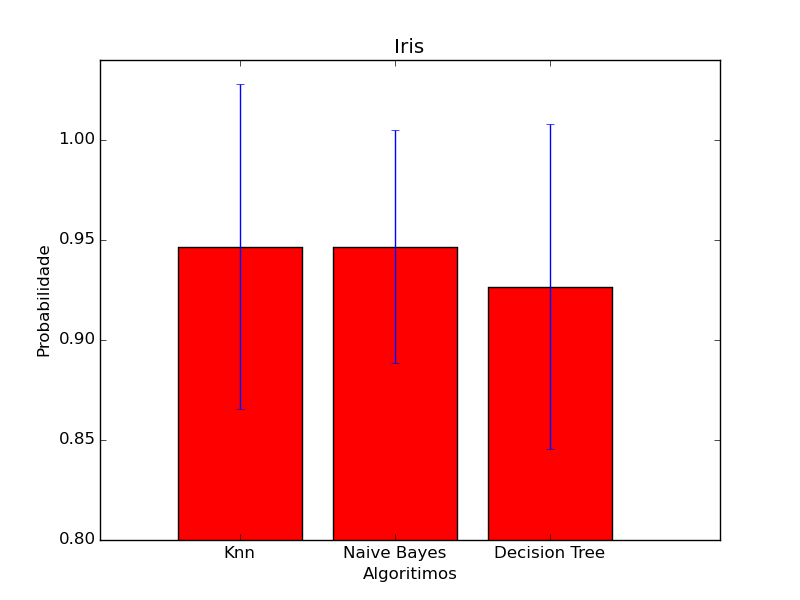
\includegraphics[width=0.35\textwidth]{Iris/acuracias.png}
    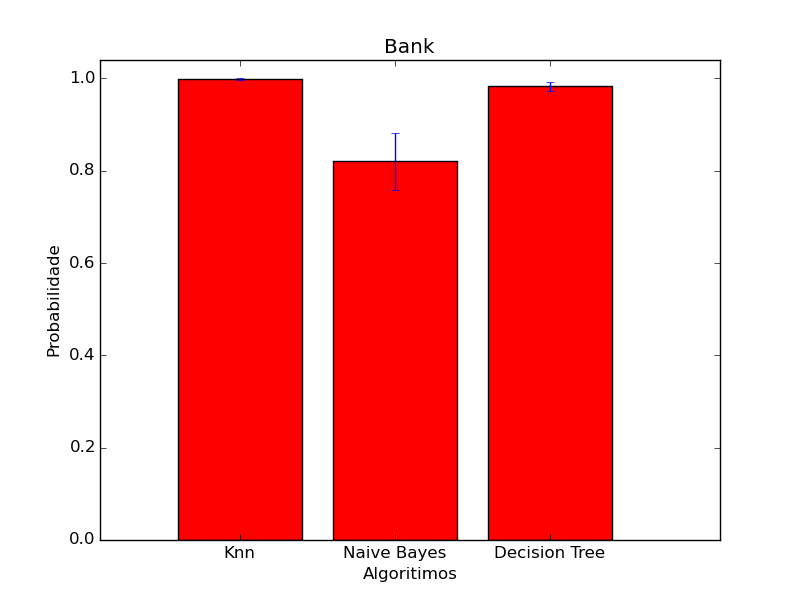
\includegraphics[width=0.35\textwidth]{banknote_authentication/acuracias.png}
    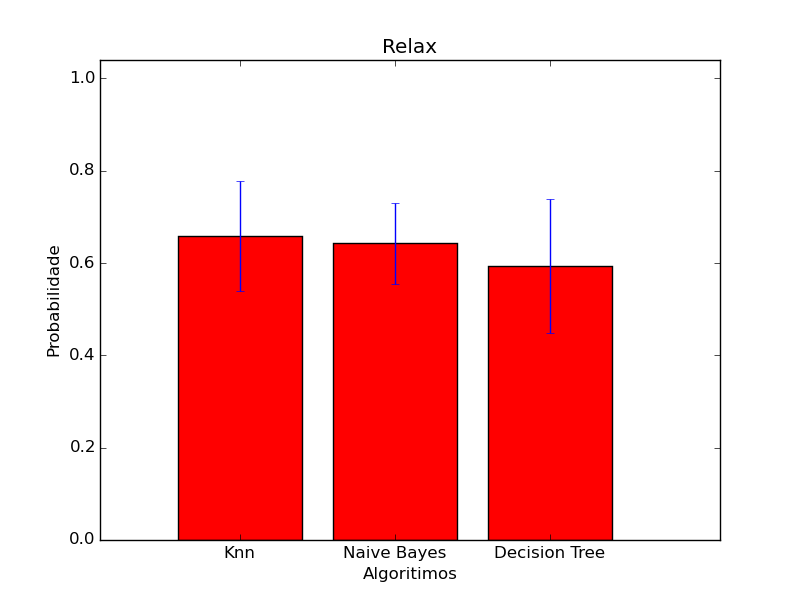
\includegraphics[width=0.35\textwidth]{Planning_Relax/acuracias.png}
    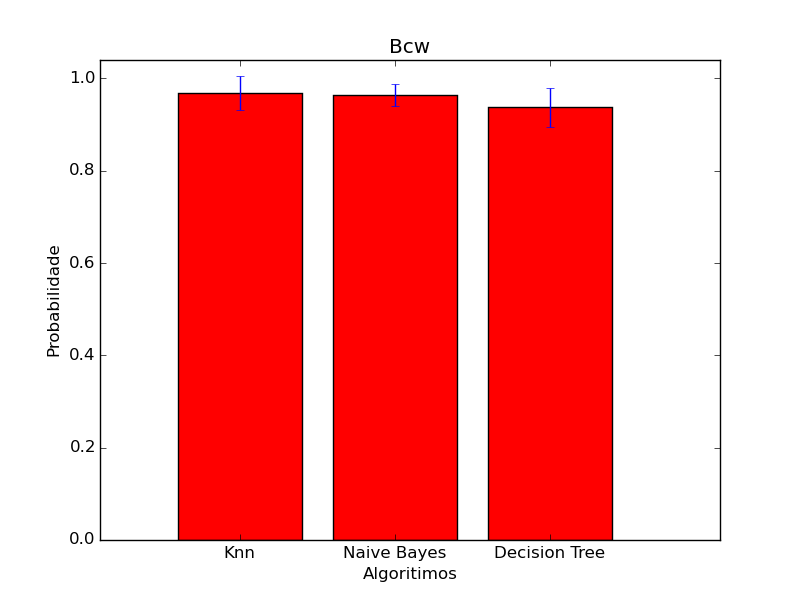
\includegraphics[width=0.35\textwidth]{Breast_Cancer/acuracias.png}
    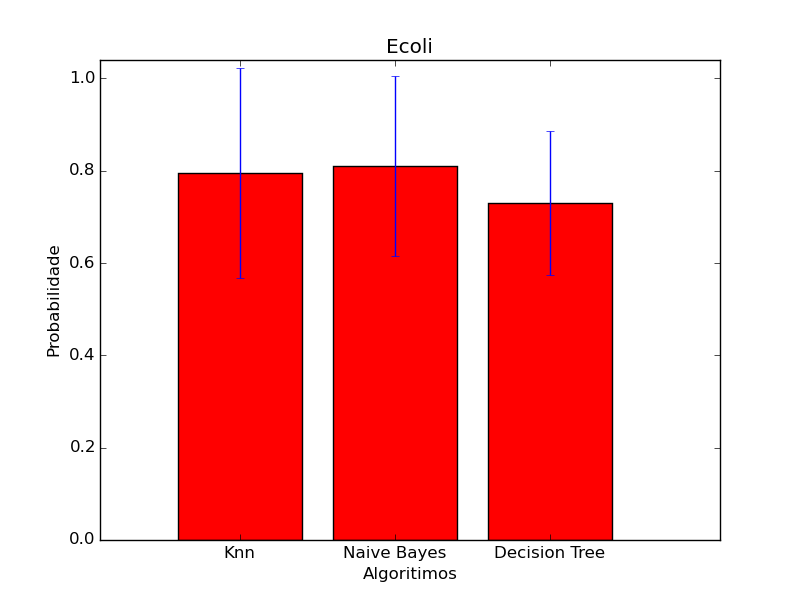
\includegraphics[width=0.35\textwidth]{ecoli/acuracias.png}
    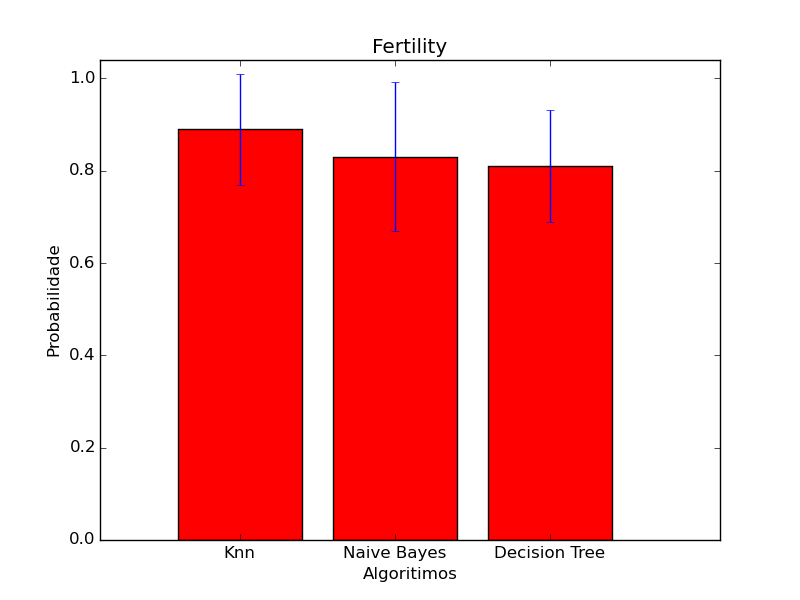
\includegraphics[width=0.35\textwidth]{fertility/acuracias.png} 
    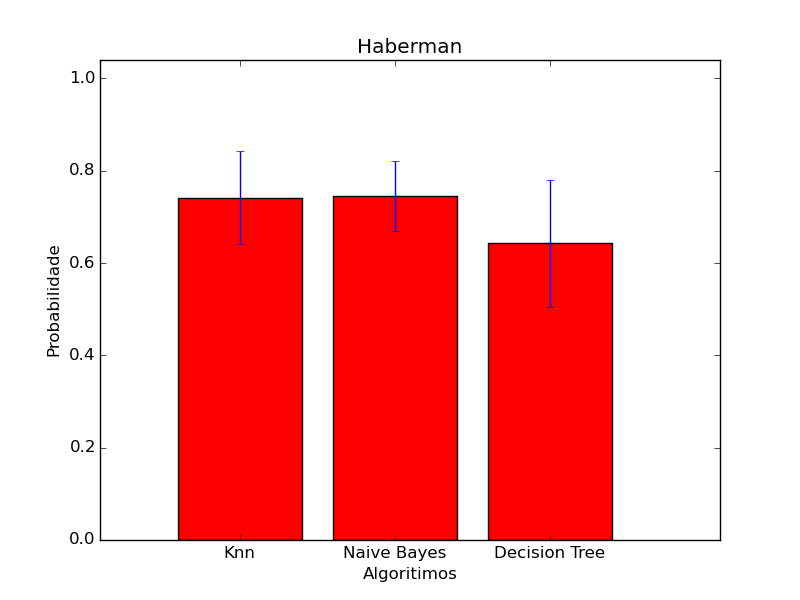
\includegraphics[width=0.35\textwidth]{Habermans_Survival/acuracias.png}    
    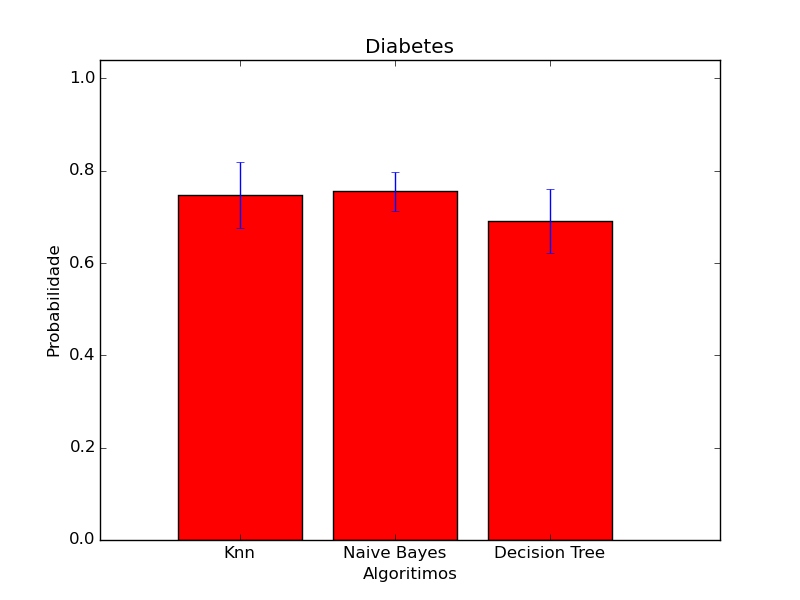
\includegraphics[width=0.35\textwidth]{Pima_Indians_Diabetes/acuracias.png}
    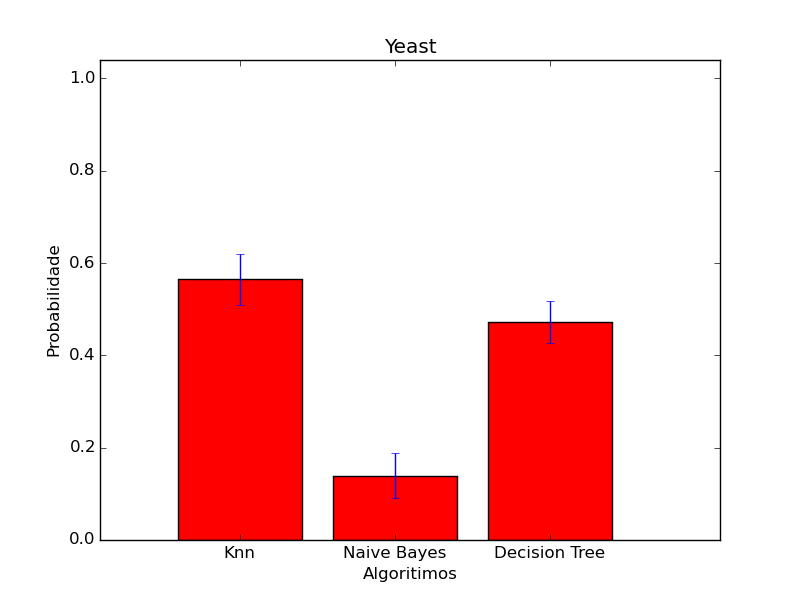
\includegraphics[width=0.35\textwidth]{Yeast/acuracias.png}
    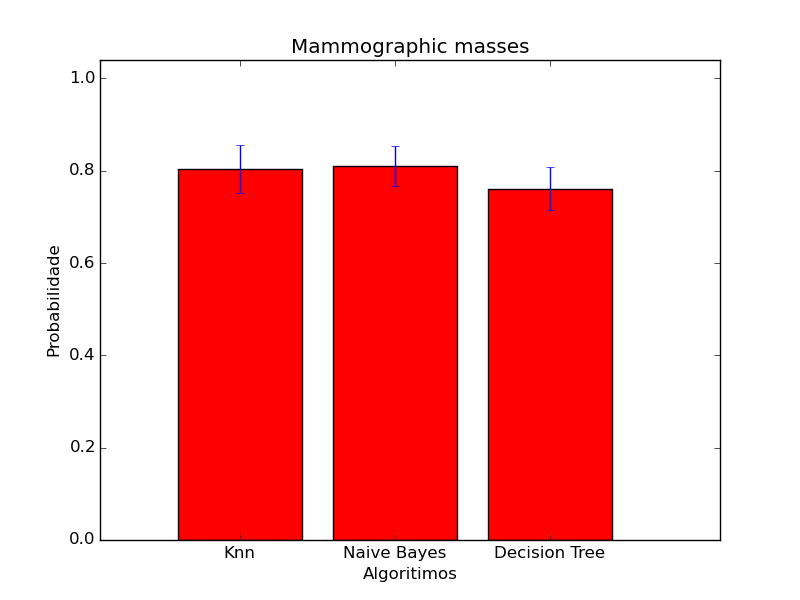
\includegraphics[width=0.35\textwidth]{Mammographic_Mass/acuracias.png}          
\end{figure}
\end{landscape}

\begin{landscape}
\begin{figure}[!htb]
\label{kknn}
  \caption{Escolha do número de vizinhos mais próximos}
  \centering
    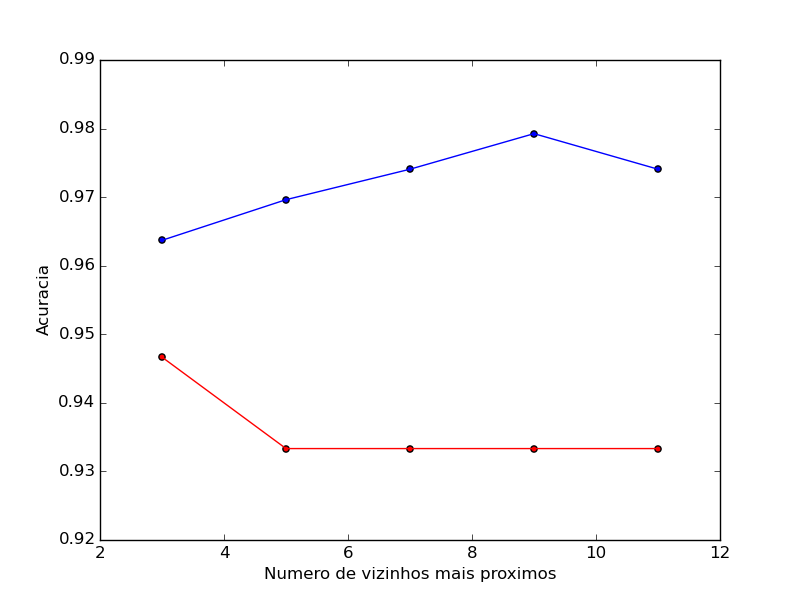
\includegraphics[width=0.35\textwidth]{Iris/knn.png}
    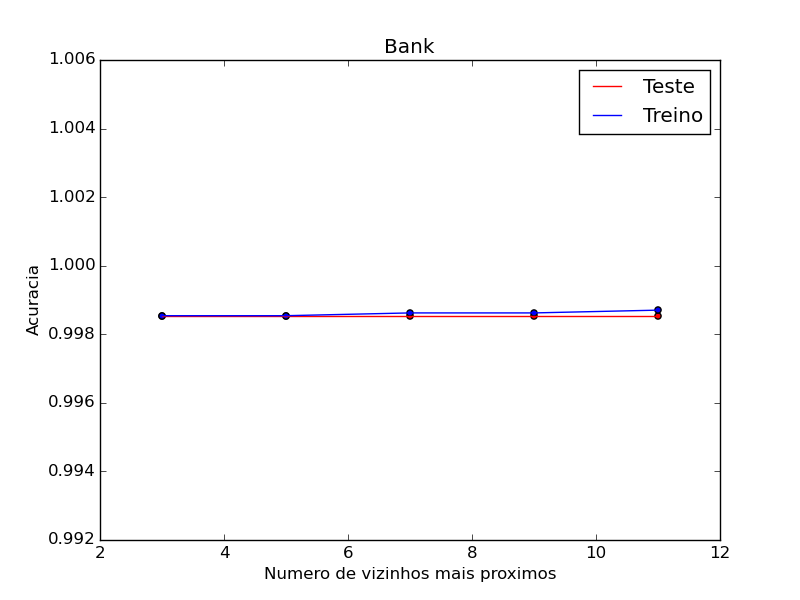
\includegraphics[width=0.35\textwidth]{banknote_authentication/knn.png}
    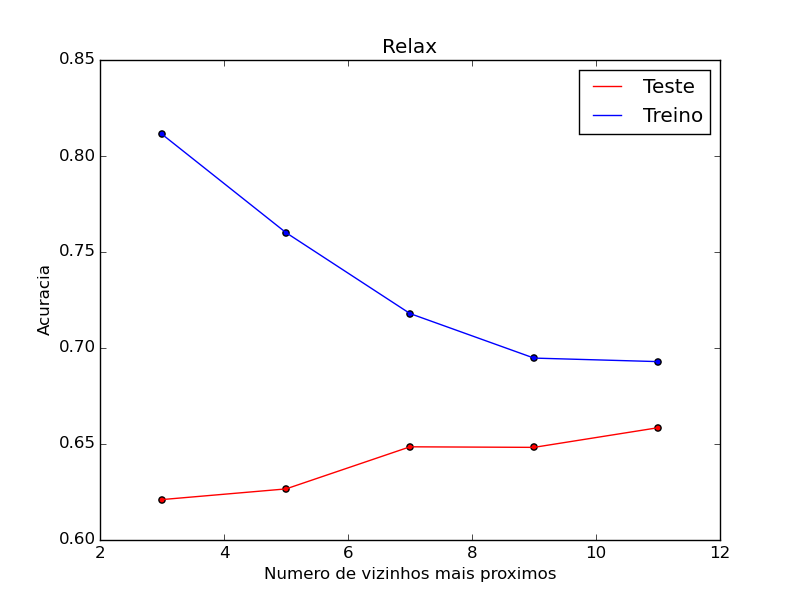
\includegraphics[width=0.35\textwidth]{Planning_Relax/knn.png}
    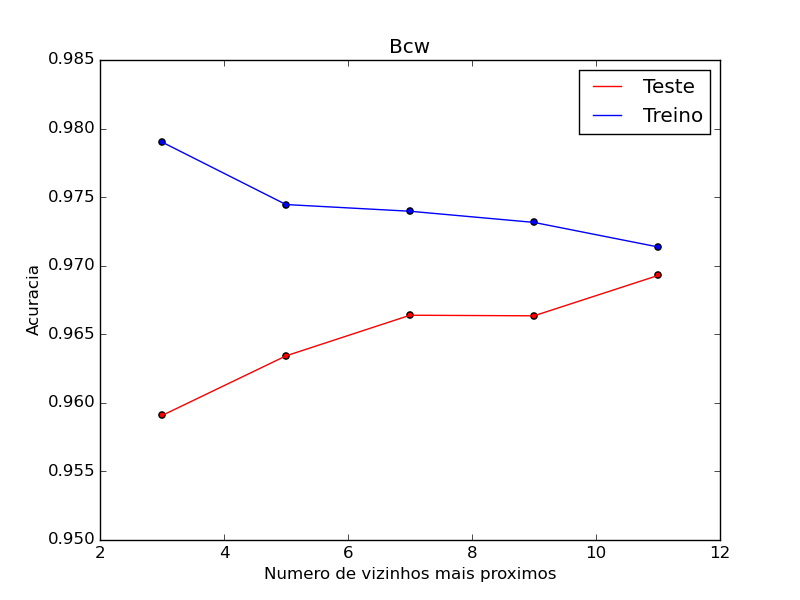
\includegraphics[width=0.35\textwidth]{Breast_Cancer/knn.png}
    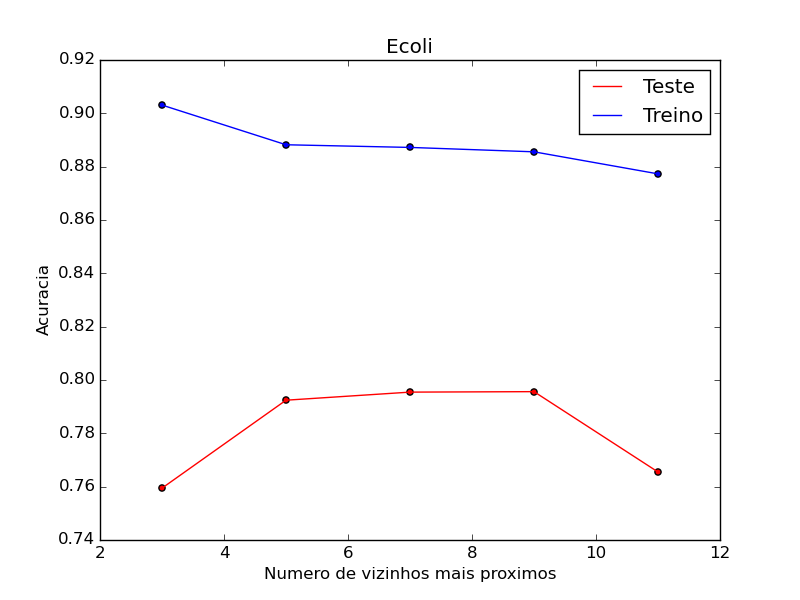
\includegraphics[width=0.35\textwidth]{ecoli/knn.png}
    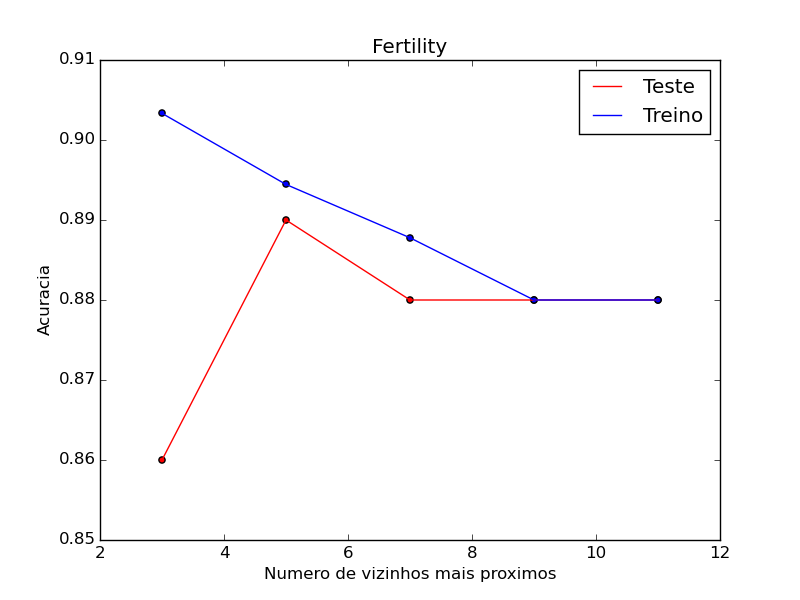
\includegraphics[width=0.35\textwidth]{fertility/knn.png} 
    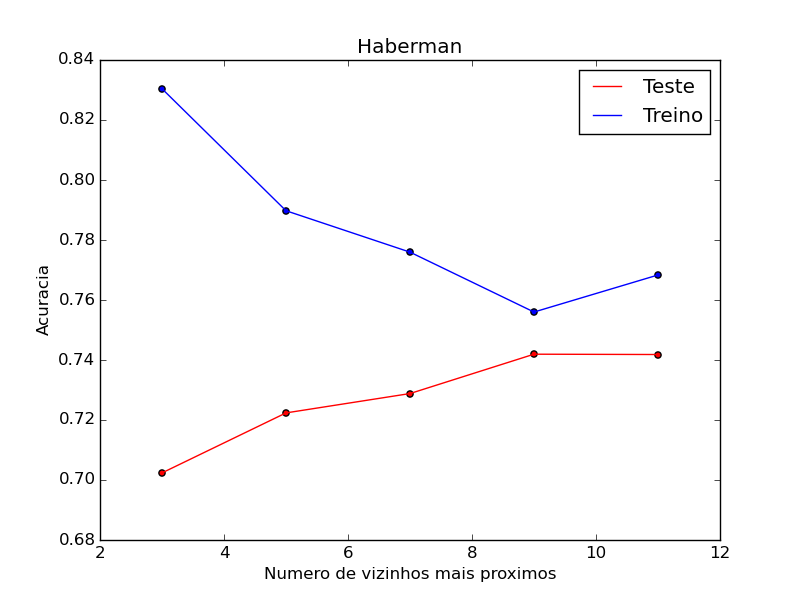
\includegraphics[width=0.35\textwidth]{Habermans_Survival/knn.png}    
    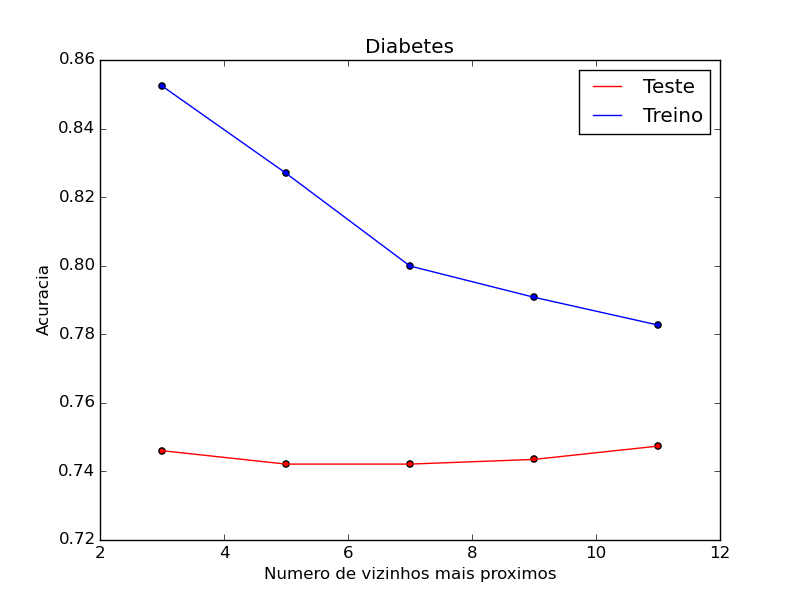
\includegraphics[width=0.35\textwidth]{Pima_Indians_Diabetes/knn.png}
    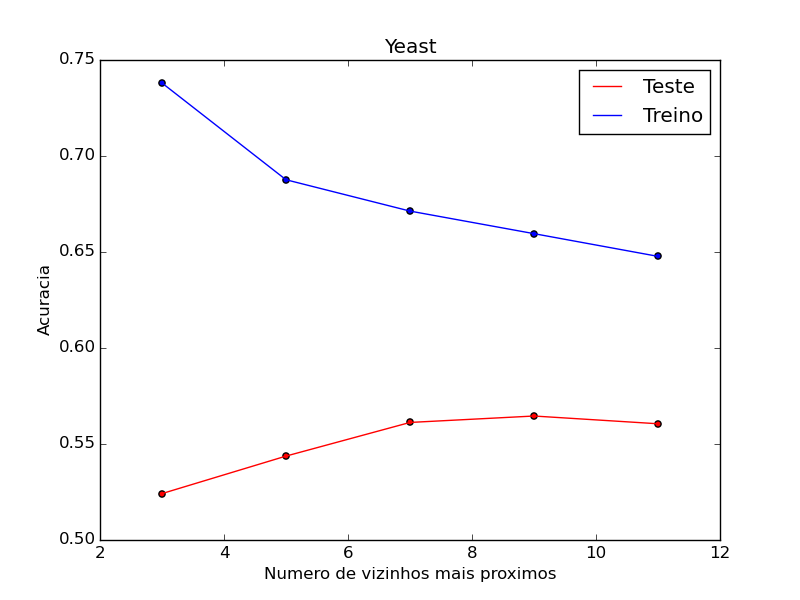
\includegraphics[width=0.35\textwidth]{Yeast/knn.png}
    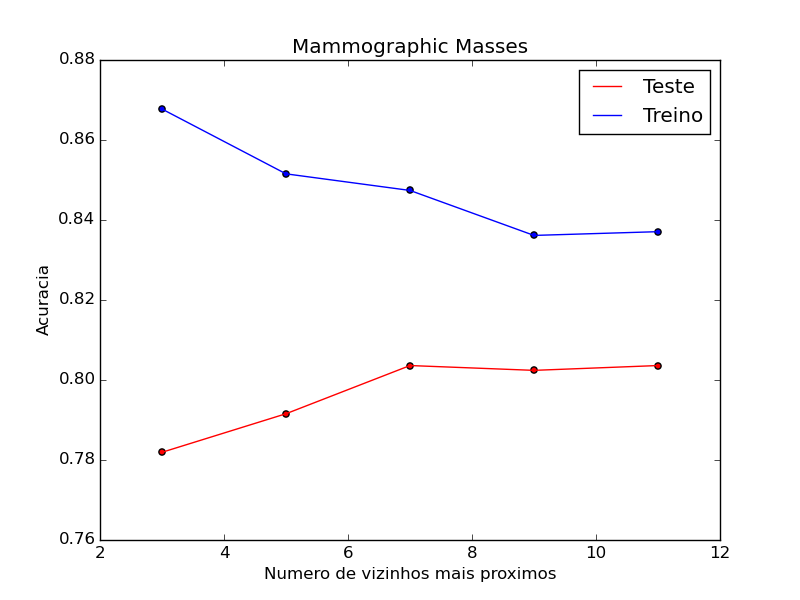
\includegraphics[width=0.35\textwidth]{Mammographic_Mass/knn.png}
\end{figure}
\end{landscape}

\begin{figure}[!htb]
  \caption{Exemplo de árvore de decisão gerada para o conjunto de dados Iris}
  \centering
  \label{arvdecisao}
    \includegraphics[width=1\textwidth]{Iris/arvore.eps}
\end{figure}

\newpage
\bibliography{Trabalho_IA.bib}

\end{document}